\setcounter{table}{0}
\begin{table}[t]
    \rowcolors{2}{gray!25}{white}
    % \setlength\arrayrulewidth{0pt}
    \centering
    \resizebox{\textwidth}{!}{%
    \begin{tabular}{ c c c c c c }
        \toprule \textbf{Language Workbench} & \textbf{Modularization Supp.} & \textbf{Precompiled Feature Supp.} & \textbf{Native IDE gen.} & \textbf{LSP/DAP Gen.} & \textbf{LSP/DAP Mod.} \\
        \midrule
        JustAdd & \LEFTcircle & \Circle & \Circle & \Circle & \Circle \\
        Melange & $\circledwedge$ & \Circle  & 3rd party (EMF) & \ding{80} & \ding{80} \\
        MontiCore & \LEFTcircle & \LEFTcircle & \CIRCLE & \Circle & \Circle \\
        MPS & $\circledwedge$ & \Circle   & \CIRCLE & \ding{80} & \ding{80} \\
        Rascal & \Circle & \Circle & \CIRCLE & \Circle & \Circle \\
        Spoofax & $\circledwedge$  & \LEFTcircle  & \CIRCLE & \ding{80} & \ding{80} \\
        Xtext & \Circle & \LEFTcircle  & \CIRCLE & \CIRCLE & \Circle \\
        Neverlang & $\circledvee$ & \CIRCLE & \Circle & \FiveStarConvex & \FiveStarConvex \\
        \bottomrule
    \end{tabular}
    }
    \caption{Comparison of language workbenches in terms of modularization, precompiled feature support, native IDE generation, LSP generation, and LSP modularization. The $\CIRCLE$ symbol indicates full support, $\Circle$ no support, $\LEFTcircle$ limited support, $\circledvee$ fine-grained modularization,  $\circledwedge$ coarse-grained modularization, \FiveStarConvex my expected contribution and \ding{80} my expected contribution that can be extended to all LWs that support at least component modularization.}
    \label{tab:lw-comparison}
\end{table}

The primary goal of this project is to develop a Universal \textbf{Language Server Protocol}\footnote{https://microsoft.github.io/language-server-protocol} (LSP) and \textbf{Debugger Adapter Protocol}\footnote{https://microsoft.github.io/debug-adapter-protocol} (DAP) for modular language workbenches (LWs). This endeavor seeks to address significant gaps and challenges developing LSPs and DAPs in the current landscape of language workbenches, particularly in the areas of modularization, composition, and interoperability. Current language workbenches such as Neverlang~\cite{Cazzola20}, Melange~\cite{Degueule15}, MontiCore~\cite{Krahn10}, Spoofax~\cite{Visser10}, and MPS~\cite{Volter11, Voelter12} have made significant strides in supporting modularization, composition, and IDE integration.
The table~\ref{tab:lw-comparison} provides a comparison of various language workbenches in terms of their support for modularization, precompiled feature support, native IDE generation, LSP generation, and LSP modularization. The $\CIRCLE$ symbol indicates full support, $\Circle$ no support, $\LEFTcircle$ limited support, $\circledvee$ fine-grained modularization, $\circledwedge$ coarse-grained modularizationand, \FiveStarConvex my expected contribution, which can be extended to all LWs that support at least component modularization (identified by \ding{80}).
The second column indicates the level of support for modularization of artifacts and language features (more detail in Project Description section), as can be see in the table~\ref{tab:lw-comparison}, Neverlang is the only LW that supports fine-grained modularization, which is essential for the development of language product lines~\cite{Cazzola21b, Cazzola15f} (LPLs). The third column indicates the level of support for precompiled features, the importance of this feature lies in the fact that an artifact can be used by several features being compiled once, and that one feature can be used among several projects without the recompilation step~\cite{Leduc20}. The fourth column indicates the level of support for native IDE generation, this is because many LWs are supported by the existence of some IDE and thus allow IDE generation for languages developed for the IDE that hosts them.
The generation and modularizazion of LSP and DAP is trivially shown by the fifth and sixth columns, respectively.
However, their approaches are often fragmented and lack a standardized method for LSP and DAP generation and modularization, as shown in Table~\ref{tab:lw-comparison}, also due to their coarse-grained modularity.
Neverlang~\cite{Cazzola15c, Cazzola14c}, developed at the \texttt{ADAPT-Lab}\footnote{https://di.unimi.it/it/ricerca/risorse-e-luoghi-della-ricerca/laboratori-di-ricerca/adapt-lab} of the Università degli Studi di Milano, being a comprehensive framework for language composition and fine-grained modularization~\cite{Cazzola15f, Cazzola21b}, is a prime candidate for the implementation of the proposed LSP and DAP. The project will leverage the existing capabilities of Neverlang to develop a universal LSP and DAP that can be used across different programming languages and IDEs. This will enable developers to create external domain-specific languages~\cite{Fowler10} (DSLs) and general-purpose languages (GPLs) more effectively and efficiently, enhancing the overall development experience and productivity. Moreover, the reusability of modules across different languages is a key feature of some LWs. By developing a core reusable base for LSP and DAP, the project will establish a foundation for creating new languages and features more efficiently. This will enable developers to leverage existing modules and components to build LSPs and DAPs for new languages more quickly and effectively, reducing development time and effort significantly.

\hfill \break
In the following, the \textbf{Research Objectives} (RO) are outlined, along with their \textbf{relevance} in the context of the state of the art. The relevance of each RO is discussed in terms of \textbf{Research Questions} (RQs) that will guide the investigation and development of the proposed universal LSP and DAP for modular language workbenches.

\hfill \break
\noindent
\textbf{\hypertarget{ro1}{RO 1}: Improve IDE and LSP Generation}
\hfill \break
\textit{Integrated Development Environment} generation and support for the \textit{Language Server Protocol} are essential for the practical use of domain-specific languages (DSLs). While some language workbenches like Xtext~\cite{Bettini13b} support LSP generation~\cite{Barros22}, many do not, limiting their usability across different editors and IDEs.
\hfill \break
% \textbf{Relevance:} By establishing a universal protocol for LSP and DAP, this project aims to bridge the gap, enabling language workbenches to generate IDE support and LSPs more seamlessly. This will ensure that languages developed using these workbenches can be used in any IDE that supports these protocols, enhancing their accessibility and utility.
\textsf{\hypertarget{rq11}{RQ 1.1}}: How can IDE generation be improved to support LSP and DAP?
\hfill \break
\textsf{\hypertarget{rq12}{RQ 1.2}}: What are the key challenges in generating LSP and DAP for different programming languages?
\hfill \break
\textsf{\hypertarget{rq13}{RQ 1.3}}: How can a universal LSP and DAP be developed to support multiple languages and IDEs?

\hfill \break
\noindent
\textbf{\hypertarget{ro2}{RO 2}: Facilitate LSP and DAP Modularization}
\hfill \break
LSP and DAP modularization are not widely supported by current language workbenches~\cite{Bunder19a}. This feature is crucial for allowing different language components to communicate and function cohesively within an IDE.
\hfill \break
% \textbf{Relevance:} Implementing support for LSP and DAP modularization will allow for better integration and interaction of various language features, thereby improving the overall development experience and capability of language workbenches. This aligns with the needs for more sophisticated and integrated language development tools as highlighted in the contemporary research and development literature.
\textsf{\hypertarget{rq21}{RQ 2.1}}: How can LSP and DAP modularization be facilitated in language workbenches?
\hfill \break
\textsf{\hypertarget{rq22}{RQ 2.2}}: What are the key challenges in modularizing LSP and DAP for different programming languages?
\hfill \break
\textsf{\hypertarget{rq23}{RQ 2.3}}: How can LSP and DAP modularization be integrated with existing language composition and modularization features in language workbenches?

\hfill \break
\noindent
\textbf{\hypertarget{ro3}{RO 3}: Reduce to $\mathbf{L} \times 1$ the number of combinations to support $\mathbf{L}$ languages}

\begin{figure}[t]
    \centering
    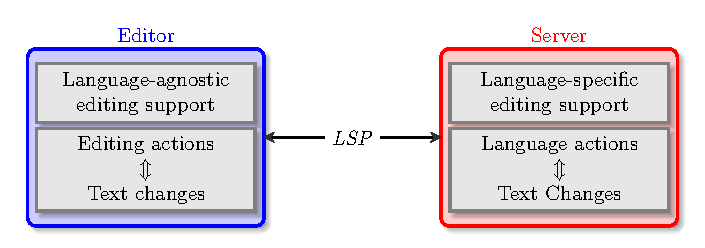
\includegraphics[width=0.75\linewidth]{figs/lsp_agnostic.pdf}
    \caption{LSP and DAP approach for programming languages (From~\cite{Rodriguez-Echeverria18a}).}
    \label{fig:agnostic}
\end{figure}

\hfill \break
Before the advent of LSP and DAP, developers had to implement language support for each editor separately, having the number of combinations to support $\mathbf{L}$ languages in $\mathbf{L} \times \mathbf{E}$, where $\mathbf{E}$ is the number of editors.
Currently, the number of combinations to support $\mathbf{L}$ languages is $\mathbf{L} + \mathbf{E}$~\cite{Rodriguez-Echeverria18a}, as the Microsoft LSP and DAP are editor-agnostic, as shown in Figure~\ref{fig:agnostic}. This project aims to reduce the number of combinations to $\mathbf{L} \times 1$, by developing a universal LSP and DAP that can be used across different programming languages and IDEs.
\hfill \break
% \textbf{Relevance:} Reducing the number of combinations required to support multiple languages will simplify the development process and make it more efficient. This will enable developers to create language support more quickly and effectively, enhancing the overall productivity and usability of language workbenches.
\textsf{\hypertarget{rq31}{RQ 3.1}}: How can the number of combinations required to support multiple languages be reduced to $\mathbf{L} \times 1$?
\hfill \break
\textsf{\hypertarget{rq32}{RQ 3.2}}: In what ways does simplifying the development process for language support enhance efficiency?
\hfill \break
\textsf{\hypertarget{rq33}{RQ 3.3}}: How does reducing combinations impact the speed and effectiveness of creating language support?

\hfill \break
\noindent
\textbf{\hypertarget{ro4}{RO 4}: Leverage Neverlang for LSP and DAP in LPL Development}
\hfill \break
Neverlang's capabilities for language composition and modularization make it an ideal platform for developing a universal LSP and DAP that caters to a variety of language needs. By leveraging Neverlang's LPL development features~\cite{Cazzola20}, the project will establish a reusable core for LSP and DAP functionalities, allowing for the creation of product line variants tailored to specific programming language requirements. This will significantly reduce development time and effort for creating LSPs and DAPs for new languages within the product line.
\hfill \break
% \textbf{Relevance:}  Developing a core reusable base for LSP and DAP functionalities through Neverlang's LPL features will streamline the creation of new language support. This fosters a more efficient and scalable approach to LSP and DAP development, aligning perfectly with the core principles of software product lines.
\textsf{\hypertarget{rq41}{RQ 4.1}}: How can Neverlang's LPL development features be leveraged for creating a reusable core for LSP and DAP functionalities?
\hfill \break
\textsf{\hypertarget{rq42}{RQ 4.2}}: What are the key benefits of using Neverlang for LSP and DAP development in the context of LPLs?
\hfill \break
\textsf{\hypertarget{rq43}{RQ 4.3}}: How does leveraging Neverlang's LPL features enhance the scalability and efficiency of LSP and DAP development?
